% T3 of the Transport Papers series.
% Correction (2026-09-10, mechanical pass, per Leon): rule 23 misidentified T5 as the printed-version exception. T1 is the exception at Version 3.0; every other paper, T5 included, reads Version 1.0. \date corrected accordingly (was 1.1).
% v1.1 (2026-09-10, derivation session, Fable 5.1 subagent, per rule 20,
%   series-review repair pass against series_review_2026-09-09.md).
%   Review 2.13: Fact 6.1 (fact:walls) now carries T4's hypotheses: the
%   radical line bundle trivial, w_1(L) = 0 (T4 Thm 4.4), for the one-sided
%   completion, totality and relocation clauses; Sigma compact (T4 Lem 5.3,
%   Cor 5.5) for the tameness of the shadow wall and the infinite wall
%   sequence, with the automatic triviality of each shadow wall's radical
%   line noted. Cor 6.2 (cor:iteration) hypothesis sentence now refers to
%   those hypotheses. Numbering unchanged.
%   Rule 18: Sec 7 (sec:position) opens "This paper is T3 of the series.";
%   T1, T4, T5, T7, T9, T12, T14 all named as "Tn \cite{ButlerTn}"; new
%   \bibitem entries for ButlerT5, T7, T9, T12, T14 with the series titles;
%   ButlerT1/T4 titles checked. Sec 6 "T5 of this series computes" -> "T5
%   \cite{ButlerT5} computes".
%   Rule 10 form: \newtheorem{fact} display name -> "Fact (imported)"; the
%   "Imported: " prefix dropped from the brackets of Facts 2.2, 3.4, 3.5,
%   5.4, 6.1. Environment types and numbering unchanged.
%   Sec 8: "from-scratch basis-blade implementation" -> the shared library's
%   product (the script imports GA.py); the capacity sentence now says the
%   isotropy and rank check runs in both Cl(2,4) and Cl(3,5), which the
%   script now does. Same docstring fix in verify_T03.py.
%   \date bumped to Version 1.1. Abstract untouched (238 words), no em dashes.
%   Script: verify_T03.py 31/31 PASS, re-run. Cl(3,5) capacity check now
%   also asserts the three creation vectors are independent (exact rank 3),
%   folded into the existing check; the Cl(1,0) odd-charge check's
%   self-commutation clause replaced by a real commutativity test (all
%   blade pairs, and two general rational elements). Count unchanged at 31.
%   Compile: pdflatex x2, 17 pages, 0 errors, 0 undefined refs, 0 multiply
%   defined, 0 overfull, no float overflow.
% 2026-09-09 addendum (interactive session with Leon, Opus 5). Two changes
%   per Leon: (1) the printed version is now 1.0 for every paper T0 to T17,
%   T5 alone at 3.0 (progress-doc rule 23); the development numbering is
%   retired from the title page and kept in this header. (2) Every reference
%   to the programme monograph is removed (rule 24), re-pointed to the series
%   where a sibling paper carries the result and otherwise restated to stand
%   alone. No mathematics, no labels and no numbering changed, so verify_T03.py
%   stands unchanged at 31/31 and was not re-run.
%   Here: the iteration question and the second-quantisation claim are the
%   paper's own; the tower-results comparison replaced by a contribution list.
% v1.2 (2026-09-09, derivation session, Fable 5.1 subagent, per rule 20, review-repair pass
% against T03_review_v1.md, same session; 0 B, 2 S, 6 N). S1: Rem 5.7 "here no choice is
% involved" (contradicted the remark's own complexification sentence) -> "here no hidden choice
% is made". S2: Section 8 "Thirty-two checks in all" -> "Thirty-one", matching the script's
% 31 PASS lines. N1: \date -> Version 1.2, September 2026. N2: Lemma 3.3 lead-in "properties
% ... is elementary" -> "are elementary and are proved". N3: Section 6.3 "used in the proofs of
% the physical papers" -> "used by the physical papers". N4: verify_T03.py check 11 (literal
% True) rebuilt: on floors 0, 1, 2 the floor volume element is computed and shown to
% anticommute with every generator, so (1 +- omega)/2 is not central and, with centre =
% span{1}, the only central idempotents are 0 and 1. N5: the v1.1 block below says "Lemma
% 2.5 title"; the lemma is 3.3 (lem:amplification). N6 (naive corrector wording) not changed.
% Check count 31 before and after (one predicate rebuilt, none added). Compile: pdflatex x2,
% 17 pages, 0 errors, 0 undefined, 0 multiply-defined, 0 overfull, no float overflow.
% Numbering frozen: aux diff empty. verify_T03.py: 31 PASS, ALL CHECKS PASSED. No knock-ons.
% v1.1 (2026-09-08, prose pass, Fable 5.1 subagent, per project rule 22: mannered prose
% replaced by literal statement, Leon's ruling to replace the recurring vocabulary too).
% Body only; version 1.0 header below untouched. Compile: pdflatex x2, 17 pages, 0 errors,
% 0 undefined references, 0 multiply-defined labels. verify_T03.py: 31 PASS before and
% after, ALL CHECKS PASSED; script unchanged. Numbering unchanged (aux diff empty).
% About 37 sentences changed. Glossary items applied: "priced" -> "quantified" (1);
% "capacity ledger" -> "capacity count" (2); "honest" dropped or replaced by "precise" /
% "the adjoint for this inner product" (3); "load-bearing" -> "used in the proofs of" (1);
% "fires" (fusion) -> "occurs" (1); "lives at" -> "lies at" (1); "killed" -> "sent to zero" (1);
% "bookkeeping" -> "computation" / "structural properties" / "description" / "directly from
% the transport construction" / "a Jordan-Wigner transformation" (5, incl. Lemma 2.5 title
% "Matrix amplification bookkeeping" -> "Matrix amplification: structural properties").
% Non-glossary: "the engine of the section" -> "the central construction"; "the series' own
% machinery" -> "results"; "standing negotiation" -> "sequence of such meetings"; "clash" ->
% "conflict"; "marching away" -> "displaced successively away"; "no ingenuity of vector choice"
% -> "no choice of vectors"; "a no-go" -> "a prohibition"; "owes the reader" -> "must state";
% "no choice is being smuggled" -> "no choice is involved"; "not the naive one" -> "differs from
% the single-step corrector"; "what the physics wanted it to be" -> "the object the physical
% reading requires"; "assert the folklore" -> "assert the unproved standard expectation";
% "the corollary the question deserved" -> "the corollary that answers the question"; "fix the
% arena" -> "fix the algebraic setting"; "algebraic home" -> "the algebra in which ... lies";
% "division of labour" -> "division"; "X's business" -> "X's task" (2); "a pointer" -> "a
% reference"; "skeleton of their constructions" -> "framework". Kept as defined names: tower,
% rung, floor, ground floor, clock/frozen clock/ticks, wall, shadow wall, register, capacity.
% Version 1.0: tower rigidity (commuting copies via x -> x Omega_k;
% Cl(k,k) = M_{2^k}(R) through T1's ladder-pair theorem), Fock modules and
% capacity, the even-charge CAR limit, the odd-charge Question, the
% iteration corollary assembling T1 + T4 + this paper. One figure (the
% tower with its one-qubit rungs, Section 2). verify_T03.py accompanies.
% 2026-08-25 review pass: matrix-unit convention fixed once (Fact 2.1);
% compatibility lemma added (the transported connecting maps carry a SPLIT
% corrector diag(u_A x 1, 1 x Omega_k), not diag(1, u_k)); *-structure and
% C*-norms of the tower defined and proved; creation/annihilation labels
% corrected (a_j = w_j annihilates the vacuum); Fact (imported) discipline
% (rule 11); Position section (rule 15).
% House rules: no em dashes; short abstract; standard series disclaimer.
\documentclass[11pt]{article}
\usepackage[margin=1.1in]{geometry}
\usepackage{amsmath,amssymb,amsthm,mathtools}
\usepackage[dvipsnames]{xcolor}
\usepackage{tikz}
\usepackage[colorlinks=true,linkcolor=MidnightBlue,citecolor=MidnightBlue,urlcolor=MidnightBlue]{hyperref}

\newtheorem{theorem}{Theorem}[section]
\newtheorem{proposition}[theorem]{Proposition}
\newtheorem{lemma}[theorem]{Lemma}
\newtheorem{corollary}[theorem]{Corollary}
\theoremstyle{definition}
\newtheorem{definition}[theorem]{Definition}
\newtheorem{remark}[theorem]{Remark}
\newtheorem{example}[theorem]{Example}
\newtheorem{question}[theorem]{Question}
\newtheorem{fact}[theorem]{Fact (imported)}

\newcommand{\Cl}{\mathrm{Cl}}
\newcommand{\R}{\mathbb{R}}
\newcommand{\C}{\mathbb{C}}
\newcommand{\HH}{\mathbb{H}}
\newcommand{\Z}{\mathbb{Z}}
\newcommand{\Mat}{\mathrm{M}}
\newcommand{\CAR}{\mathrm{CAR}}
\newcommand{\UHF}{\mathrm{UHF}}
\newcommand{\End}{\mathrm{End}}
\newcommand{\Ad}{\mathrm{Ad}}

\title{\bfseries The Tower and the CAR Limit\\[4pt]
  \large\itshape Iterated Transport, the Frozen Clock, and Second Quantisation}
\author{Leon Butler\\ \normalsize\href{mailto:lbutler.math@gmail.com}{\texttt{lbutler.math@gmail.com}}\\ \normalsize ORCID: \href{https://orcid.org/0009-0006-4449-5617}{0009-0006-4449-5617}}
\date{Version 1.0, September 2026 \textperiodcentered{} Transport Papers, T3}

\begin{document}
\maketitle

\begin{abstract}
\normalsize
The transport principle of this series completes $\Cl(p,q)$ to $\Cl(p{+}1,q{+}1)$; the completed algebra carries a null cone of its own, so the completion invites iteration. This paper settles what the iterated tower is. Rigidity first: $\Cl(p{+}k, q{+}k) \cong \Mat_{2^k}(\Cl(p,q))$ canonically, so the transport charge $p - q$ is constant along the tower and the mod-8 clock never ticks. Bott periodicity manifests not as eventual return but as immediate freeze: every floor is Morita equivalent to the ground floor, and the eight clock positions classify eight parallel towers rather than stages of one. Each rung adjoins one hyperbolic plane, and the adjoined ladder pairs satisfy the canonical anticommutation relations exactly, as vectors: the tower is a fermionic register, one mode per rung, with Fock modules doubling at every floor and the Witt index counting capacity. The limit theorem settles the second-quantisation question: for even transport charge the grade twist in the connecting embeddings is inner by Skolem and Noether, the algebraic direct limit is $\Cl(p,q) \otimes \Mat_{2^\infty}$, and the completed complexified limit is the ground algebra tensored with the CAR algebra of countably many fermionic modes. Iterated transport is second quantisation. The odd-charge case, where the twist acts on the centre, is delimited precisely and posed. The paper is pure mathematics: complete proofs throughout, with the handful of imported classical results stated as facts carrying their provenance. Every computational identity is verified in exact arithmetic in an accompanying script.
\end{abstract}

\medskip
\noindent\textbf{MSC 2020.} Primary 15A66, 46L05; Secondary 46L60, 81R10, 15A63.\\
\textbf{Keywords.} Clifford algebra; Witt completion; matrix amplification; mod-8 periodicity; CAR algebra; UHF algebra; second quantisation; Fock space.

\newpage
\textbf{Authorship and disclosure. }The founding idea of the series is the author's: that division by zero in a Clifford algebra should be read not as a prohibition but as a transport into a higher-dimensional algebra, and that the transported division need not be accompanied by an inverse operation. The direction of investigation and the critical review of the results are likewise the author's. The mathematical development and the drafting of the text were carried out in extended collaboration with Claude Fable 5 (Anthropic), an AI system.

\newpage
\section{Introduction}\label{sec:intro}

The root paper of the series \cite{ButlerT1} repairs the failure of division at the null cone of $\Cl(p,q)$ by the minimal Witt completion $\Cl(p,q) \to \Cl(p{+}1,q{+}1)$, shows this is one of exactly two transport rules, classifies what each adjoins, and proves that the completed algebra is the matrix amplification $\Mat_2(\Cl(p,q))$ with the base embedded as a twisted diagonal. The completed algebra, being a Clifford algebra of mixed signature, has a null cone of its own. The question this paper answers is the evident one: what happens when the transport is iterated? Three specific forms of the question: does the ascended algebra's own singular behaviour force a further ascent, without end; does the mod-8 periodicity of the real Clifford classification make the climb circulate; and what is the limit object?

The answers are more specific than the questions. The tower $\Cl(p{+}k,q{+}k)$ is canonically $\Mat_{2^k}(\Cl(p,q))$, so the climb never leaves the ground floor's Morita class: the clock is frozen, not circulating, and the eight clock positions classify eight parallel towers, one per transport charge $p - q \bmod 8$, rather than eight stages of one tower. What the iteration accumulates is capacity, not algebraic type: each rung adjoins one hyperbolic plane whose ladder pair satisfies the canonical anticommutation relations exactly, the Fock module doubles, and the Witt index, the algebra's count of independent fermionic modes, increases by exactly one. The limit is then the object the physical reading requires: the ground algebra tensored with the CAR algebra of a free fermionic field. Iterated transport is second quantisation, one mode per rung.

The mathematical content of the limit statement requires operator-algebraic care, which it receives here. The connecting embeddings are twisted diagonals $a \mapsto \operatorname{diag}(a, \hat a)$, with $\hat a$ the grade involution; whether the twist can be removed decides whether the limit is a plain tensor product. For even transport charge the ground algebra is central simple, the involution is inner by the Skolem-Noether theorem, and the twist conjugates away rung by rung: the algebraic limit is exactly $\Cl(p,q) \otimes \Mat_{2^\infty}$, and its completed complexification is $\Cl(p,q)_\C \otimes \CAR$. For odd charge the grade involution acts nontrivially on the centre and is outer; the even-charge argument does not apply, and rather than assert the unproved standard expectation we delimit the boundary and pose the odd case precisely.

\subsection*{Prior art}

Every ingredient is classical; the assembly and the transport reading are the contributions. The isomorphism $\Cl(p{+}1,q{+}1) \cong \Mat_2(\Cl(p,q))$ is the $(1,1)$-periodicity of the real Clifford classification, due in matrix form to the classical structure theory \cite{Porteous1995, Lounesto2001} and in K-theoretic form to Atiyah, Bott and Shapiro \cite{ABS1964}; \cite{ButlerT1} re-derives it directly from the transport construction, with the ladder pair as explicit matrix units, and that derivation is the one iterated here. UHF algebras and their classification are Glimm's \cite{Glimm1960}; AF algebras and their diagrams are Bratteli's \cite{Bratteli1972}; the CAR algebra, its uniqueness, its Fock representations and its identification with the $2^\infty$ UHF algebra are standard operator algebra \cite{BratteliRobinson1997}. The Chevalley construction realising Clifford algebras on exterior algebras of isotropic subspaces \cite{Chevalley1997} is the mechanism behind the Fock module theorem. The Skolem-Noether theorem, the classical frame for the even-charge innerness \cite{Pierce1982}, is not actually imported: the implementing element is exhibited directly. Morita theory is classical \cite{Lam1999}. The infinite wall sequence that makes the far-side iteration unconditional is proved in the sheaf paper of this series \cite{ButlerT4}; the root paper \cite{ButlerT1} supplies the single step and its minimality. The contributions here are the canonical form of the rigidity, the exact CAR relations at vector level, the Skolem-Noether treatment of the grade twist, and the precise odd-charge boundary.

\subsection*{Contribution}

At the standard of \cite{ButlerT1}: complete proofs, each theorem carrying its own hypotheses.

\begin{enumerate}
\item \textbf{Tower rigidity} (Section \ref{sec:rigidity}). $\Cl(p{+}k,q{+}k) \cong \Mat_{2^k}(\Cl(p,q))$ by an isomorphism assembled canonically from the $k$ ladder pairs, with the commuting-copies mechanism made explicit: the base re-embeds as $x \mapsto x\,\omega_1\cdots\omega_k$ against the adjoined planes' volume elements, and the two constructions (nested matrix units, commuting copies) agree. Transport charge is invariant, the clock is frozen, every floor is Morita equivalent to the ground floor, and no type-C obstruction ever arises by transport from a simple ground algebra.
\item \textbf{Eight towers} (Section \ref{sec:rigidity}). The mod-8 residues classify parallel towers; a signature-change wall is a meeting of two towers whose charges differ by two, and the shadow-wall phenomenon of \cite{ButlerT4} is re-read as tower change.
\item \textbf{One qubit per rung} (Section \ref{sec:fock}). The adjoined null pairs satisfy the CAR exactly as vectors; the Fock module theorem: the algebra of $k$ adjoined planes acts irreducibly on the exterior algebra of the span of the creation directions, of dimension $2^k$, doubling per rung; and Witt index is quantum capacity: the maximal number of independent fermionic modes an algebra of the tower hosts is exactly its Witt index, which increases by one per rung.
\item \textbf{The CAR limit} (Section \ref{sec:limit}). For $p - q$ even: the grade involution is inner (Skolem-Noether), the twisted diagonals conjugate to untwisted ones stage by stage, the algebraic direct limit of the tower is $\Cl(p,q) \otimes \Mat_{2^\infty}$ canonically, and the completed complexified limit is $\Cl(p,q)_\C \otimes \CAR$, the ground algebra tensored with a free fermionic field algebra. For $p - q$ odd the twist is outer on the centre and the question is posed with the obstruction identified.
\item \textbf{What the dynamics demands} (Section \ref{sec:reading}). Imported from \cite{ButlerT4} and \cite{ButlerT1} and assembled: on the physical closure nothing divides by zero at floor one and no further ascent is dynamically forced; beyond the shadow walls the demand is unconditional and infinite, one rung per wall. The scope section separates algebra-level theorems from physical readings.
\end{enumerate}


\section{Setup: the tower}\label{sec:setup}

\subsection{The single step, recalled}\label{subsec:step}

Throughout, $\Cl(p,q)$ is the real Clifford algebra of the nondegenerate form of signature $(p,q)$ on $\R^n$, $n = p + q$, with mixed signature $p, q \geq 1$ where null vectors are in question; notation follows \cite{ButlerT1}. Rule 1, the Witt completion, adjoins a hyperbolic plane $H = \operatorname{span}\{e, f\}$ with $e^2 = 1$, $f^2 = -1$, $e \cdot f = 0$, equivalently a null pair $v = \tfrac12(e+f)$, $w = \tfrac12(e-f)$ with $v^2 = w^2 = 0$ and $v \cdot w = \tfrac12$. The ladder pair $(v, w)$ satisfies
\begin{equation}\label{eq:car1}
vw + wv = 1, \qquad v^2 = w^2 = 0,
\end{equation}
and generates, with the base, the completed algebra $\Cl(p{+}1, q{+}1)$. The single step is imported once, with its matrix-unit labelling fixed for the whole paper:

\begin{fact}[The single step is matrix amplification]\label{fact:step}
Let $A$ be the Clifford algebra of a base quadratic space and $(v, w)$ the null pair of an adjoined hyperbolic plane, normalised as in \eqref{eq:car1}. Then
\[
E_{12} := v, \qquad E_{21} := w, \qquad E_{11} := vw, \qquad E_{22} := wv
\]
are a $2 \times 2$ matrix-unit system with $E_{11} + E_{22} = 1$; the corner $E_{11}\, \Cl'\, E_{11}$ of the completed algebra $\Cl'$ is $A \cdot E_{11}$; the resulting identification $\Cl' \cong \Mat_2(A)$ embeds the base as the twisted diagonal $a \mapsto \operatorname{diag}(a, \hat a)$, with $\hat a$ the grade involution of $A$; and in these units the adjoined plane's volume element is $\omega = ef = wv - vw = \operatorname{diag}(-1, +1)$. \emph{Provenance:} \cite[Thm.~7.1]{ButlerT1}. Which of $vw$, $wv$ is called $E_{11}$ is a convention; this paper uses the displayed labelling throughout, and Lemma \ref{lem:compat} records where the choice matters.
\end{fact}

\begin{definition}[The tower]\label{def:tower}
The \emph{tower} over $\Cl(p,q)$ is the chain of algebras $T_k := \Cl(p{+}k, q{+}k)$, $k \geq 0$, on the spaces $\R^{p,q} \perp H_1 \perp \cdots \perp H_k$ with $H_j = \operatorname{span}\{e_j, f_j\}$ orthogonal hyperbolic planes, together with the natural unital embeddings $\iota_k : T_k \hookrightarrow T_{k+1}$ induced by the inclusion of quadratic spaces. Write $v_j, w_j$ for the $j$-th null pair, $\omega_j := e_j f_j$ for the $j$-th plane's volume element, and $d := p - q \bmod 8$ for the \emph{transport charge}.
\end{definition}

\begin{remark}[Why this tower]\label{rem:whytower}
Rule 1 is the only rule that iterates: by \cite[Prop.~7.4]{ButlerT1} the fusion rule occurs at most once along any transport history and a pure Rule-1 lineage stays fusion-free, so the minimal repeated completion is exactly Definition \ref{def:tower}. Minimality and uniqueness at each step are \cite[Thm.~4.13]{ButlerT1}, so the tower is the canonical iterated repair, not one choice among many.
\end{remark}

\begin{figure}[t]
\centering
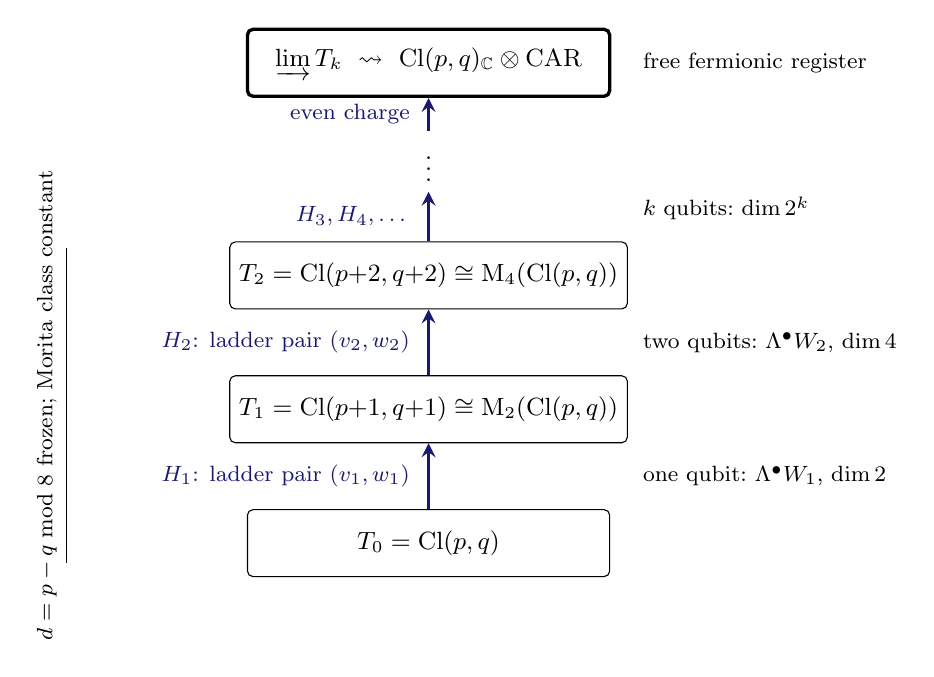
\begin{tikzpicture}[>=stealth, yscale=1.0,
  floor/.style={draw, rounded corners=2pt, minimum width=4.6cm, minimum height=8.5mm, font=\small},
  rung/.style={->, very thick, MidnightBlue},
  note/.style={font=\footnotesize, align=left}]
\node[floor] (t0) at (0,0) {$T_0 = \Cl(p,q)$};
\node[floor] (t1) at (0,1.7) {$T_1 = \Cl(p{+}1,q{+}1) \cong \Mat_2(\Cl(p,q))$};
\node[floor] (t2) at (0,3.4) {$T_2 = \Cl(p{+}2,q{+}2) \cong \Mat_4(\Cl(p,q))$};
\node[font=\small] (dots) at (0,4.85) {$\vdots$};
\node[floor, very thick] (lim) at (0,6.1) {$\varinjlim T_k \ \leadsto\ \Cl(p,q)_\C \otimes \CAR$};
\draw[rung] (t0) -- (t1) node[midway, left, note, xshift=-1mm] {$H_1$: ladder pair $(v_1, w_1)$};
\draw[rung] (t1) -- (t2) node[midway, left, note, xshift=-1mm] {$H_2$: ladder pair $(v_2, w_2)$};
\draw[rung] (t2) -- (dots) node[midway, left, note, xshift=-1mm] {$H_3, H_4, \dots$};
\draw[rung] (dots) -- (lim) node[midway, left, note, xshift=-1mm] {even charge};
\node[note, anchor=west] at (2.6,0.85) {one qubit:\ $\Lambda^\bullet W_1$, $\dim 2$};
\node[note, anchor=west] at (2.6,2.55) {two qubits:\ $\Lambda^\bullet W_2$, $\dim 4$};
\node[note, anchor=west] at (2.6,4.25) {$k$ qubits:\ $\dim 2^k$};
\node[note, anchor=west] at (2.6,6.1) {free fermionic register};
\draw[thin] (-4.6,-0.25) -- (-4.6,3.75) node[midway, rotate=90, above, font=\footnotesize] {$d = p - q \bmod 8$ frozen; Morita class constant};
\end{tikzpicture}
\caption{The tower and its rungs. Each floor $T_k = \Cl(p{+}k, q{+}k)$ is obtained from the one below by adjoining a single hyperbolic plane $H_k$ (Definition \ref{def:tower}), whose null ladder pair $(v_k, w_k)$ satisfies the canonical anticommutation relations exactly, as vectors (Proposition \ref{prop:car}): one fermionic mode, one qubit, per rung. Algebraically each rung is the matrix amplification $\Mat_2$ (Theorem \ref{thm:commuting}), so the transport charge $d$ and the entire Morita class are constant along the climb (Theorem \ref{thm:rigidity}): the clock is frozen, and the mod-8 residues label eight parallel towers rather than stages of one. The Fock module doubles per rung (Theorem \ref{thm:fock}), and for even charge the completed complexified limit is the ground algebra tensored with the CAR algebra of countably many modes (Theorem \ref{thm:carlimit}).}
\label{fig:tower}
\end{figure}

\section{Tower rigidity: the frozen clock}\label{sec:rigidity}

The central construction of the section is a pair of commuting subalgebras that between them generate each floor. The construction is classical in spirit; the form given here keys it to the transport data (the planes and their volume elements), which is what makes the iteration and the limit computation of Section \ref{sec:limit} exact. Figure \ref{fig:tower} displays the object the section is about.

\begin{lemma}[Volume elements of the planes]\label{lem:volumes}
Let $\omega_j = e_j f_j$. Then $\omega_j^2 = 1$; $\omega_j$ anticommutes with $e_j$ and $f_j$; $\omega_j$ commutes with $e_i, f_i$ for $i \neq j$ and with every ground generator; and the $\omega_j$ commute pairwise. Hence $\Omega_k := \omega_1 \cdots \omega_k$ satisfies $\Omega_k^2 = 1$, commutes with all ground generators, and anticommutes with each $e_j, f_j$, $j \leq k$.
\end{lemma}

\begin{proof}
$\omega_j^2 = e_j f_j e_j f_j = -e_j^2 f_j^2 = -(1)(-1) = 1$, using $f_j e_j = -e_j f_j$. $\omega_j e_j = e_j f_j e_j = -e_j^2 f_j = -f_j$ while $e_j \omega_j = e_j e_j f_j = f_j$: they anticommute, and likewise for $f_j$. A ground generator or a generator of another plane anticommutes with both letters of $\omega_j$, hence commutes with their product. Pairwise commutation of the $\omega_j$ is the same parity count. The $\Omega_k$ statements follow: against $e_j$, exactly one factor ($\omega_j$) anticommutes.
\end{proof}

\begin{theorem}[Commuting copies]\label{thm:commuting}
Inside $T_k$, let $B_k$ be the subalgebra generated by the $2k$ plane generators $e_1, f_1, \dots, e_k, f_k$, and let $A_k$ be the subalgebra generated by the twisted base generators $x^{(k)} := x\,\omega_1 \omega_2 \cdots \omega_k$ for $x$ among the ground generators. Then: $B_k \cong \Cl(k,k) \cong \Mat_{2^k}(\R)$; $A_k \cong \Cl(p,q)$ via $x \mapsto x^{(k)}$ (the twisted generators satisfy the ground Clifford relations); $A_k$ and $B_k$ commute elementwise; and multiplication $A_k \otimes B_k \to T_k$ is an isomorphism of algebras,
\[
\Cl(p{+}k, q{+}k) \;\cong\; \Cl(p,q) \otimes \Mat_{2^k}(\R) \;=\; \Mat_{2^k}(\Cl(p,q)).
\]
The isomorphism is canonical given the ordered planes, and compatible with the tower embeddings up to the twist tracked in Section \ref{sec:limit}.
\end{theorem}

\begin{proof}
\emph{$B_k \cong \Cl(k,k)$.} The $2k$ generators are orthonormal for the split form ($e_j^2 = 1$, $f_j^2 = -1$, pairwise orthogonal), so the universal property gives a surjection $\Cl(k,k) \to B_k$; it is injective because the $2^{2k}$ blades in the letters $e_1, f_1, \dots, e_k, f_k$ are part of the blade basis of $T_k$, hence independent. \emph{$\Cl(k,k) \cong \Mat_{2^k}(\R)$} by induction using the series' own results: $\Cl(0,0) = \R$, and $\Cl(j{+}1,j{+}1) \cong \Mat_2(\Cl(j,j))$ is Fact \ref{fact:step} with base $\Cl(j,j)$, the $(j{+}1)$-st plane carrying the outer index, so $\Cl(k,k) \cong \Mat_2(\Mat_2(\cdots)) = \Mat_{2^k}(\R)$.

\emph{$A_k \cong \Cl(p,q)$.} By Lemma \ref{lem:volumes}, $\Omega_k$ commutes with ground generators and $\Omega_k^2 = 1$, so for ground generators $x, y$:
\[
x^{(k)} y^{(k)} + y^{(k)} x^{(k)} = x \Omega_k y \Omega_k + y \Omega_k x \Omega_k = (xy + yx)\,\Omega_k^2 = 2B(x,y) .
\]
The universal property gives an algebra map $\Cl(p,q) \to A_k$, $x \mapsto x^{(k)}$; it sends the base blade $x_I$ to $x_I\,\Omega_k^{|I| \bmod 2}$, and these images are distinct nonzero blades (times a fixed invertible even element), hence independent: the map is an isomorphism onto $A_k$.

\emph{Commutation.} For a ground generator $x$ and any plane generator $g \in \{e_j, f_j\}$: $x$ anticommutes with $g$, and $\Omega_k$ anticommutes with $g$ (Lemma \ref{lem:volumes}), so $x^{(k)} g = x \Omega_k g = -x g \Omega_k = g x \Omega_k = g x^{(k)}$. Generators commute, hence the subalgebras do.

\emph{Multiplication is an isomorphism.} Commutation makes $A_k \otimes B_k \to T_k$ an algebra map. It is surjective: its image contains every plane generator, contains $\Omega_k \in B_k$, and therefore contains each ground generator $x = x^{(k)} \Omega_k$. Source and target both have dimension $2^n \cdot 2^{2k} = 2^{n + 2k}$, so a surjective linear map is an isomorphism. Finally $\Cl(p,q) \otimes \Mat_{2^k}(\R) = \Mat_{2^k}(\Cl(p,q))$. Canonicity: the construction used only the ordered orthogonal planes and their volume elements, no basis choices in the ground algebra. The compatibility with $\iota_k$ is Lemma \ref{lem:twist} below: under these identifications $\iota_k$ is the twisted diagonal, the twist being conjugation by $\Omega$-data that Section \ref{sec:limit} tracks.
\end{proof}

The structural properties of matrix amplification, used repeatedly below, are elementary and are proved here once; the one genuinely imported piece of Morita theory is stated as a fact.

\begin{lemma}[Matrix amplification: structural properties]\label{lem:amplification}
Let $A$ be a unital real algebra and $m \geq 1$. Then: (i) $Z(\Mat_m(A)) = Z(A)\cdot 1_m$; (ii) if $A$ is simple, so is $\Mat_m(A)$; (iii) $\Mat_m(\Mat_r(D)) \cong \Mat_{mr}(D)$ for any unital $D$; (iv) $\Mat_m(A_1 \oplus A_2) \cong \Mat_m(A_1) \oplus \Mat_m(A_2)$.
\end{lemma}

\begin{proof}
(i) Let $z = (z_{ij})$ be central. The entries of $z E_{kl} = E_{kl} z$ are $(z E_{kl})_{ij} = z_{ik}\,\delta_{lj}$ and $(E_{kl} z)_{ij} = \delta_{ik}\, z_{lj}$; equality for all $i, j, k, l$ forces $z_{ik} = 0$ for $i \neq k$ and $z_{kk} = z_{ll}$, so $z = a \cdot 1_m$ with $a := z_{11}$, and commuting with $b \cdot 1_m$ for all $b \in A$ forces $a \in Z(A)$. The converse inclusion is clear. (ii) A nonzero two-sided ideal $I$ contains some $x$ with an entry $x_{kl} = a \neq 0$; then $E_{ik}\, x\, E_{lj} = a E_{ij} \in I$ for all $i, j$, so $I \supseteq \Mat_m(AaA) = \Mat_m(A)$, since $AaA = A$ by simplicity. (iii) and (iv) are regroupings of indices and entrywise splittings.
\end{proof}

\begin{fact}[Morita equivalence of an algebra and its amplification]\label{fact:morita}
For any unital ring $A$ and $m \geq 1$, the column module $A^m$ is a $\Mat_m(A)$-$A$-bimodule implementing an equivalence of module categories: $A$ and $\Mat_m(A)$ are Morita equivalent. \emph{Provenance:} classical Morita theory, \cite[\S\S 17--18]{Lam1999}.
\end{fact}

\begin{fact}[The type-C diagnosis]\label{fact:typeC}
A real Clifford algebra carries a type-C obstruction exactly when its centre contains a nontrivial idempotent, that is, when the centre is $\R \oplus \R$. \emph{Provenance:} \cite[Thm.~3.6]{ButlerT1}.
\end{fact}

\begin{theorem}[Rigidity; the clock is frozen]\label{thm:rigidity}
Along the tower: the transport charge $d = p - q \bmod 8$ is constant; the division-ring type, simplicity class, and centre of every floor equal those of the ground floor; every floor is Morita equivalent to the ground floor; and the obstruction taxonomy of \cite{ButlerT1} is floor-independent: in particular a type-C obstruction (a central idempotent) never arises by transport from a simple ground algebra, at any height. The physical tower is $\Cl(1{+}k, 3{+}k) \cong \Mat_{2^{k+1}}(\HH)$, frozen at clock position $6$. Bott periodicity manifests as immediate freeze, not eventual return.
\end{theorem}

\begin{proof}
The charge is $(p{+}k) - (q{+}k) = p - q$, constant. All structural claims then follow from Theorem \ref{thm:commuting} and Lemma \ref{lem:amplification}: centres agree by (i); if $A \cong \Mat_r(D)$ then $\Mat_{2^k}(A) \cong \Mat_{2^k r}(D)$ by (iii), the same division ring; simplicity propagates by (ii), and the block structure of a semisimple ground floor by (iv); and every floor is Morita equivalent to the ground floor by Fact \ref{fact:morita}. The taxonomy statement: by Fact \ref{fact:typeC}, type C occurs exactly when the centre is $\R \oplus \R$; the centre is floor-independent by Lemma \ref{lem:amplification}(i), so a simple ground floor (centre $\R$ or $\C$) propagates: no floor of its tower ever hosts a type-C obstruction. For the physical case, $\Cl(1,3) \cong \Mat_2(\HH)$ \cite{Porteous1995}, so floor $k$ is $\Mat_{2^k}(\Mat_2(\HH)) = \Mat_{2^{k+1}}(\HH)$, and $1 - 3 \equiv 6 \pmod 8$.
\end{proof}

\begin{remark}[Eight towers; signature change is tower change]\label{rem:eighttowers}
The eight clock positions classify not stages of one tower but eight parallel towers, one per transport charge. The two sides of a tame signature-change wall carry charges $d$ and $d - 2$ \cite[\S 7.2]{ButlerT4}, and the shadow wall, where the two competing completions conflict, is where two towers of different charge meet. The wall sequence of \cite[Cor.~5.5]{ButlerT4} is a sequence of such meetings between neighbouring towers, displaced rung by rung away from the physical region.
\end{remark}

\section{One qubit per rung: Fock modules and capacity}\label{sec:fock}

\begin{proposition}[The ladder pairs satisfy the CAR, as vectors]\label{prop:car}
In $T_k$, the adjoined null pairs satisfy, exactly and at the level of vectors,
\[
v_i v_j + v_j v_i = 0, \qquad w_i w_j + w_j w_i = 0, \qquad v_i w_j + w_j v_i = \delta_{ij}\,,
\]
for all $1 \leq i, j \leq k$: a system of $k$ fermionic modes, with no normal-ordering, no completion, and no representation chosen. Adding a rung adds one mode and touches none of the existing relations.
\end{proposition}

\begin{proof}
Every displayed relation is an instance of the single Clifford relation $\alpha\beta + \beta\alpha = 2\langle\alpha, \beta\rangle$ on vectors: the $v$'s are pairwise orthogonal null vectors ($\langle v_i, v_j \rangle = 0$ for $i \neq j$ since the planes are orthogonal, and $v_i^2 = 0$ since $v_i$ is null), likewise the $w$'s, and $\langle v_i, w_j \rangle = \tfrac12\delta_{ij}$ by the hyperbolic normalisation within each plane and orthogonality across planes. A new rung's vectors are orthogonal to all previous generators, so the old relations are untouched.
\end{proof}

\begin{theorem}[Fock module; one qubit per rung]\label{thm:fock}
Let $W_k := \operatorname{span}\{v_1, \dots, v_k\}$, a maximal isotropic subspace of $H_1 \perp \cdots \perp H_k$. The Chevalley action ($v_j$ by wedge, $w_j$ by contraction against the pairing) makes the exterior algebra $\Lambda^\bullet W_k$, of dimension $2^k$, an irreducible module over $B_k \cong \Mat_{2^k}(\R)$, with the vacuum $1 \in \Lambda^0$ annihilated by every $w_j$ and cyclic for the $v_j$. Each rung doubles the module: $\Lambda^\bullet W_{k+1} = \Lambda^\bullet W_k \otimes \Lambda^\bullet \R v_{k+1}$, one qubit per rung.
\end{theorem}

\begin{proof}
\emph{The action.} $W_k$ is isotropic (Proposition \ref{prop:car}) of dimension $k$, maximal since the split form $H_1 \perp \cdots \perp H_k$ has Witt index $k$. Define, for $\xi \in \Lambda^\bullet W_k$,
\[
c(v_j)\,\xi = v_j \wedge \xi, \qquad c(w_j)\,\xi = \iota_{\varphi_j}\,\xi, \qquad \varphi_j := 2\langle w_j, \cdot\,\rangle|_{W_k} \in W_k^* ,
\]
so $\varphi_j(v_i) = \delta_{ij}$, and extend linearly to arbitrary vectors $\alpha = \sum_j (a_j v_j + b_j w_j)$.

\emph{The three anticommutator families,} elementary and proved outright. Wedge operators square to zero and pairwise anticommute, since $v \wedge v' = -v' \wedge v$ and $v \wedge v = 0$. The contraction $\iota_\varphi$ acts on monomials by
\[
\iota_\varphi(u_1 \wedge \cdots \wedge u_s) \;=\; \sum_{i=1}^{s} (-1)^{i-1}\, \varphi(u_i)\; u_1 \wedge \cdots \widehat{u_i} \cdots \wedge u_s .
\]
Two contractions anticommute: in $\iota_\varphi \iota_\psi + \iota_\psi \iota_\varphi$ applied to a monomial, the term deleting $u_j$ then $u_i$ (with $i < j$) in the first composite carries the sign
\[
(-1)^{j-1}(-1)^{i-1},
\qquad \text{against} \qquad
(-1)^{i-1}(-1)^{j-2}
\]
for the matching term of the second composite, which deletes $u_i$ then $u_j$; the shift by one arises because removing $u_i$ first moves $u_j$ up a slot, and the opposite signs cancel the terms pairwise. The mixed anticommutator: the displayed expansion gives $\iota_\varphi(v \wedge \xi) = \varphi(v)\,\xi - v \wedge \iota_\varphi(\xi)$ (the $i = 1$ term, then the rest), so $\{v \wedge \cdot\,,\, \iota_\varphi\} = \varphi(v)\,\mathrm{id}$.

\emph{The Clifford relation, and the isomorphism.} Combining the three families,
\[
c(\alpha)^2 = \Bigl(\sum_j b_j \varphi_j\Bigr)\Bigl(\sum_i a_i v_i\Bigr)\,\mathrm{id} = \sum_j a_j b_j\,\mathrm{id} = \langle \alpha, \alpha\rangle\,\mathrm{id},
\]
since $\langle\alpha,\alpha\rangle = \sum_j 2 a_j b_j \langle v_j, w_j\rangle = \sum_j a_j b_j$. By the universal property $c$ extends to an algebra map $B_k \to \End(\Lambda^\bullet W_k)$. It is unital and nonzero with simple source ($B_k \cong \Mat_{2^k}(\R)$, Theorem \ref{thm:commuting}), hence injective; source and target both have dimension $2^{2k} = (2^k)^2$, so it is an isomorphism, and the module is irreducible.

\emph{Vacuum, cyclicity, doubling.} The vacuum $1 \in \Lambda^0$ is sent to zero by every contraction and generates everything under wedges: $v_{i_1} \wedge \cdots \wedge v_{i_r} = c(v_{i_1}) \cdots c(v_{i_r})\,1$. The doubling statement is the exterior algebra of a direct sum.
\end{proof}

\begin{theorem}[Witt index is quantum capacity]\label{thm:capacity}
For any nondegenerate real quadratic space $(V, Q)$, the maximal number of pairwise-anticommuting fermionic mode pairs realisable by \emph{vectors} of $\Cl(V, Q)$ (families $(a_i, b_i)$ of vectors satisfying the displayed CAR of Proposition \ref{prop:car}) is exactly the Witt index $\min(p,q)$ of $Q$. Along the tower the Witt index is $\min(p,q) + k$: each rung raises the algebra's mode capacity by exactly one, and by no more.
\end{theorem}

\begin{proof}
\emph{Upper bound.} Let $(a_i, b_i)_{i \leq m}$ be vectors satisfying the CAR. Reading the relations through the Clifford relation on vectors: $\langle a_i, a_j \rangle = 0$ for all $i, j$ (including $i = j$), and $\langle a_i, b_j \rangle = \tfrac12 \delta_{ij}$. The span of the $a_i$ is therefore totally isotropic, and the $a_i$ are independent: a vanishing combination $\sum c_i a_i = 0$ pairs against $b_j$ to give $c_j/2 = 0$. So $m \leq$ the maximal totally isotropic dimension, which for a nondegenerate real form of signature $(p,q)$ is $\min(p,q)$: diagonalise, $V = P \perp N$ with $P$ positive definite of dimension $p$ and $N$ negative definite of dimension $q$; a totally isotropic $U$ meets $P$ trivially (a nonzero $v \in U \cap P$ would have $Q(v,v) > 0$ and $Q(v,v) = 0$ at once), so the projection $U \to N$ along $P$ is injective and $\dim U \leq q$; symmetrically $\dim U \leq p$; and $\min(p,q)$ is attained by the null spans of $\min(p,q)$ hyperbolic pairs (the classical bound, cf.\ \cite[Ch.~I]{Lam2005}).

\emph{Attainment.} Split off $\min(p,q)$ orthogonal hyperbolic planes from $(V, Q)$ (Witt decomposition) and take their normalised null pairs, as in Proposition \ref{prop:car}. Along the tower, the form of signature $(p{+}k, q{+}k)$ has Witt index $\min(p,q) + k$, and each rung contributes its own plane to the attaining family.
\end{proof}

\begin{remark}[What the capacity theorem forbids]\label{rem:capacityforbids}
The theorem is a prohibition as much as a count: no choice of vectors extracts $\min(p,q) + k + 1$ fermionic modes from floor $k$. Capacity is quantified by the Witt index, the same quantity that the transport rules increment; the reading of the increment as ``one qubit per rung'' is therefore an exact identity, not an analogy. (Mode systems built from non-vector elements are a different question, deliberately outside the theorem's hypotheses; at vector level the count is sharp.)
\end{remark}

\section{The CAR limit}\label{sec:limit}

\begin{lemma}[The grade twist, and when it is inner]\label{lem:twist}
Under the isomorphism of Theorem \ref{thm:commuting}, the tower embedding $\iota_k$ becomes the twisted diagonal $a \mapsto \operatorname{diag}(a, \hat a)$ of \cite[Thm.~7.1]{ButlerT1}. If $p - q$ is even, $\Cl(p,q)$ is central simple over $\R$, the grade involution is an $\R$-algebra automorphism fixing the centre, and it is inner, implemented by the ground volume element $u$ (which anticommutes with vectors precisely when $n$ is even): $\hat a = u a u^{-1}$. Consequently $\operatorname{diag}(a, \hat a) = U \operatorname{diag}(a, a)\, U^{-1}$ with $U = \operatorname{diag}(1, u)$: the twist conjugates away at the level of the single step. (How the correction transports through the identifications of Theorem \ref{thm:commuting}, which is what the limit theorem needs, is Lemma \ref{lem:compat}; the stagewise corrector is \emph{not} simply this $U$.) If $p - q$ is odd the grade involution acts nontrivially on the centre ($\R \oplus \R$ or $\C$) and is outer; no inner correction exists.
\end{lemma}

\begin{proof}
The matrix form of $\iota_k$ is Fact \ref{fact:step} applied with base $T_k$: the new plane's ladder pair supplies the matrix units, and the base embeds as $a \mapsto \operatorname{diag}(a, \hat a)$, the grade involution taken in $T_k$. Note the parity is stable: $\dim$ of floor $k$ is $n + 2k$, of the same parity as $n$, so ``even charge'' is a property of the whole tower.

Even charge: $n$ even makes $\Cl(p,q)$ (and every floor) central simple over $\R$ \cite{Porteous1995, Lounesto2001}. The grade involution is an $\R$-algebra automorphism fixing the centre $\R$ pointwise, so its innerness is an instance of the Skolem-Noether theorem \cite{Pierce1982}; nothing need be imported, because the implementing element is exhibited directly: the volume element $u = x_1 \cdots x_n$ of an orthogonal generator frame satisfies $u x = (-1)^{n-1} x u = -xu$ for each generator $x$ (move $x$ through $n$ letters, one coincidence), and $u^2 = \pm 1$ is invertible; so $\Ad_u(x) = u x u^{-1} = -x = \hat x$ on generators, and two automorphisms agreeing on generators agree. The displayed conjugation is then the block computation $U \operatorname{diag}(a,a)\, U^{-1} = \operatorname{diag}(a, u a u^{-1})$ with $U = \operatorname{diag}(1, u)$, invertible in $\Mat_2(T_k)$.

Odd charge: the centre of each floor is $\R \oplus \R$ ($d \equiv 1 \bmod 4$) or $\C$ ($d \equiv 3 \bmod 4$), generated by $1$ and the volume element $\omega$, which is odd (its length $n + 2k$ is odd) and is therefore sent by the grade involution to $-\omega$: the involution exchanges the two central idempotents $\tfrac12(1 \pm \omega)$, respectively conjugates the central complex structure. An inner automorphism fixes the centre pointwise; the grade involution does not, so it is outer, and no unitary correction of the diagonal exists.
\end{proof}

The limit theorem compares the tower not with itself but with its image under the identifications $\varphi_k$ of Theorem \ref{thm:commuting}, and the corrector must be computed \emph{after} that transport. The next lemma does so; the answer differs from the single-step corrector.

\begin{lemma}[Compatibility: the connecting maps, transported]\label{lem:compat}
Let $p - q$ be even, $A := \Cl(p,q)$, and let $\varphi_k : T_k \to A \otimes \Mat_{2^k}(\R)$ be the identifications of Theorem \ref{thm:commuting}, with every plane's matrix units labelled as in Fact \ref{fact:step} and the planes nested in order, the $(k{+}1)$-st plane carrying the outer index of $\Mat_{2^{k+1}} = \Mat_2(\Mat_{2^k})$. Write $\theta_k(z) := z \otimes 1_{2 \times 2}$ for block doubling in the outer index, $u_A \in A$ for the ground volume element, and $\overline\Omega_k \in \Mat_{2^k}(\R)$ for the image of $\Omega_k = \omega_1 \cdots \omega_k$. Then the transported connecting map $\psi_k := \varphi_{k+1} \circ \iota_k \circ \varphi_k^{-1}$ is
\[
\psi_k \;=\; \Ad(V_k) \circ \theta_k, \qquad
V_k \;:=\; \begin{pmatrix} u_A \otimes 1_{2^k} & 0 \\ 0 & 1_A \otimes \overline\Omega_k \end{pmatrix},
\]
with $V_k$ invertible ($u_A^2 = \pm 1$, $\Omega_k^2 = 1$). The corrector is \emph{not} the transported single-step corrector $\operatorname{diag}(1, u_{T_k})$ of Lemma \ref{lem:twist}: transporting through $\varphi$ splits the correction across the two tensor legs, the ground volume acting in the first corner and the planes' volume in the second. The labelling convention of Fact \ref{fact:step} matters here: exchanging $vw$ and $wv$ exchanges the two corners of $V_k$.
\end{lemma}

\begin{proof}
Both sides are unital algebra maps into $A \otimes \Mat_{2^{k+1}}$, so it suffices to check them on generators of $A \otimes \Mat_{2^k}$: the elements $x \otimes 1$ for ground generators $x$, and $1 \otimes b$ for $b$ the image of a plane generator $g \in \{e_j, f_j\}$, $j \leq k$.

\emph{Ground generators.} $\varphi_k^{-1}(x \otimes 1) = x^{(k)} = x\,\Omega_k$. In $T_{k+1}$, $\Omega_{k+1} = \Omega_k\, \omega_{k+1}$ and $\omega_{k+1}^2 = 1$ give $x^{(k)} = x^{(k+1)}\, \omega_{k+1}$. Under $\varphi_{k+1}$, $x^{(k+1)} \mapsto x \otimes 1_{2^{k+1}}$ by definition, and $\omega_{k+1} \mapsto 1_A \otimes \operatorname{diag}(-1_{2^k}, +1_{2^k})$ by Fact \ref{fact:step} for the outer plane. Hence
\[
\psi_k(x \otimes 1) \;=\; x \otimes \operatorname{diag}(-1_{2^k},\, +1_{2^k}).
\]
On the other side, $\theta_k(x \otimes 1) = x \otimes 1_{2^{k+1}}$, and conjugating cornerwise by $V_k$: the first corner gives $(u_A \otimes 1)(x \otimes 1)(u_A \otimes 1)^{-1} = u_A x u_A^{-1} \otimes 1 = -x \otimes 1$ (Lemma \ref{lem:twist}, $n$ even), the second gives $(1 \otimes \overline\Omega_k)(x \otimes 1)(1 \otimes \overline\Omega_k)^{-1} = x \otimes 1$. The two sides agree.

\emph{Plane generators.} $\varphi_k^{-1}(1 \otimes b) = g$ and $\iota_k(g) = g \in B_{k+1}$. The nesting embeds $B_k$ into $\Mat_2(B_k)$ as the twisted diagonal of Fact \ref{fact:step} with base $B_k = \Cl(k,k)$: $g \mapsto \operatorname{diag}(g, \hat g)$, with $\hat{\cdot}$ the grade involution of $B_k$, which by Lemma \ref{lem:volumes} is implemented by $\Omega_k$ (it anticommutes with every plane generator and squares to one). Under $\varphi_{k+1}$ this reads
\[
\psi_k(1 \otimes b) \;=\; 1 \otimes \operatorname{diag}\bigl(b,\ \overline\Omega_k\, b\, \overline\Omega_k^{-1}\bigr),
\]
and conjugating $\theta_k(1 \otimes b) = 1 \otimes \operatorname{diag}(b, b)$ cornerwise by $V_k$ gives exactly the same: the first corner commutes with $u_A \otimes 1$, the second is conjugated by $\overline\Omega_k$. The two sides agree.

Two unital algebra maps agreeing on a generating set agree, and $V_k$ is invertible as stated. One full stage of this identity, with the corrector exactly as displayed, is verified in exact arithmetic over the ground algebra $\Cl(1,1)$ in the script (Section \ref{sec:verification}).
\end{proof}

\begin{theorem}[The algebraic limit, even charge]\label{thm:alglimit}
Let $p - q$ be even. The algebraic direct limit of the tower $(T_k, \iota_k)$ is canonically isomorphic to
\[
\varinjlim T_k \;\cong\; \Cl(p,q) \otimes \Mat_{2^\infty}, \qquad \Mat_{2^\infty} := \varinjlim \Mat_{2^k}(\R) \ \ (m \mapsto \operatorname{diag}(m,m)),
\]
the ground algebra tensored with the algebraic $2^\infty$ matrix algebra. Equivalently, $\varinjlim T_k$ is the Clifford algebra of the infinite-dimensional quadratic space $\R^{p,q} \perp H_1 \perp H_2 \perp \cdots$.
\end{theorem}

\begin{proof}
Write $A := \Cl(p,q)$, let $\varphi_k : T_k \to A \otimes \Mat_{2^k}$ be the isomorphisms of Theorem \ref{thm:commuting}, and transport the connecting maps: $\psi_k := \varphi_{k+1} \circ \iota_k \circ \varphi_k^{-1}$. By Lemma \ref{lem:compat},
\[
\psi_k \;=\; \Ad(V_k) \circ \theta_k, \qquad \theta_k(z) := z \otimes 1_{\,2 \times 2}\ \text{(block doubling)},
\]
with $V_k$ the split corrector displayed there. The comparison system is $(A \otimes \Mat_{2^k},\, \theta_k)$, whose limit is $A \otimes \Mat_{2^\infty}$ by definition. Intertwine the two systems stagewise: set $W_0 := 1$ and recursively $W_{k+1} := \theta_k(W_k)\, V_k^{-1}$, each $W_k$ an invertible element of $A \otimes \Mat_{2^k}$, and define $\lambda_k := \Ad(W_k)$. Then
\[
\lambda_{k+1} \circ \psi_k = \Ad(W_{k+1}) \circ \Ad(V_k) \circ \theta_k = \Ad(\theta_k(W_k)) \circ \theta_k = \theta_k \circ \Ad(W_k) = \theta_k \circ \lambda_k ,
\]
using $\theta_k \circ \Ad(W_k) = \Ad(\theta_k(W_k)) \circ \theta_k$ (a unital homomorphism carries conjugation to conjugation by the image). The squares commute exactly, so the $\lambda_k$ assemble into an isomorphism of the direct limits: $\varinjlim T_k \cong A \otimes \Mat_{2^\infty}$.

For the second description: the algebraic direct limit of Clifford algebras of a nested chain of quadratic spaces along the induced embeddings is the Clifford algebra of the union (both sides satisfy the same universal property for the union space, and every element of either side lies at a finite stage). Canonicity: the $\varphi_k$ and the correcting elements $W_k$ are built from the ordered planes and volume elements only.
\end{proof}

Completing in a C*-norm presupposes a *-structure, and a proof must state which one is meant; the tower carries a canonical one, determined by its frames.

\begin{lemma}[The *-structure of the tower, and its C*-norms]\label{lem:cstar}
Fix the tower's frames: an orthogonal ground frame $x_1, \dots, x_n$ diagonalising $Q$, and the plane frames $e_j, f_j$. On each complexified floor $T_k^{\,\C}$ there is a unique conjugate-linear antiautomorphism $*$ with $x^* = x$ for every frame generator with $x^2 = 1$ and $x^* = -x$ for every frame generator with $x^2 = -1$. Under it: every frame generator, every blade in the frame, and every ground or plane volume element is unitary ($z^* z = 1$); the ladder pairs are mutually adjoint, $v_j^* = w_j$; the connecting maps $\iota_k$, the identifications $\varphi_k$ of Theorem \ref{thm:commuting}, the block doublings $\theta_k$, and the correctors $V_k$ and $W_k$ of Lemma \ref{lem:compat} and Theorem \ref{thm:alglimit} are all compatible with $*$ (the maps are *-homomorphisms, the correctors unitary). If moreover $p - q$ is even, each $T_k^{\,\C}$ is *-isomorphic to $\Mat_{2^{m/2}}(\C)$, $m := n + 2k$, with $*$ the conjugate transpose; consequently each floor carries a unique C*-norm, every unital *-monomorphism between floors is isometric, and the increasing union $\bigcup_k T_k^{\,\C}$ carries a unique C*-norm.
\end{lemma}

\begin{proof}
\emph{Existence and uniqueness.} Renormalise the $m$ frame generators of floor $k$ to $y_i := x_i$ when $x_i^2 = 1$ and $y_i := i\,x_i$ when $x_i^2 = -1$, so that $y_i^2 = 1$ and the $y_i$ pairwise anticommute. Reversal, the unique real antiautomorphism of a Clifford algebra fixing its generating vectors (the universal property applied to the opposite algebra), extends conjugate-linearly to $T_k^{\,\C}$; call the extension $*$. It is conjugate-linear and antimultiplicative by construction, fixes each $y_i$, and on the original generators unwinds to exactly the displayed values: for $x^2 = -1$, $x = -i\,y$ gives $x^* = \overline{(-i)}\, y^* = i\,y = -x$. Uniqueness holds because a conjugate-linear antiautomorphism is determined by its values on the generators.

\emph{Unitarity and adjoint pairs.} $y_i^* y_i = y_i^2 = 1$, and each original generator satisfies $x^* x = 1$ in both cases ($x^2 = 1$ gives $x^*x = x^2 = 1$; $x^2 = -1$ gives $x^*x = -x^2 = 1$). A product of unitaries is unitary by telescoping, $(z_1 \cdots z_s)^* (z_1 \cdots z_s) = z_s^* \cdots z_1^* z_1 \cdots z_s = 1$; blades, the ground volume $u_A$, the plane volumes $\omega_j$ and $\Omega_k$, hence the corners of $V_k$, hence $V_k$ and recursively $W_k$, are such products or diagonals of them. The ladder pairs: $v_j^* = \tfrac12(e_j + f_j)^* = \tfrac12(e_j - f_j) = w_j$. The maps: $\iota_k$ and $\theta_k$ send frame generators to frame generators or to $z \otimes 1$, so they intertwine the $*$'s; for $\varphi_k$, equip $A \otimes \Mat_{2^k}(\C)$ with the tensor $*$ (the ground $*$ on $A$, conjugate transpose on matrices) and check generators: $(x\,\Omega_k)^* = \Omega_k^*\, x^* = x^* \Omega_k$ since each $\omega_j^* = f_j^* e_j^* = (-f_j)(e_j) = e_j f_j = \omega_j$ and $\Omega_k$ commutes with ground generators, matching $(x \otimes 1)^* = x^* \otimes 1$; and the matrix units of Fact \ref{fact:step} satisfy $E_{12}^* = v^* = w = E_{21}$ and $E_{11}^* = (vw)^* = w^* v^* = vw = E_{11}$, matching the conjugate transpose, nested stage by stage.

\emph{The even case is a matrix *-algebra.} Let $m$ be even and represent on $(\C^2)^{\otimes m/2}$ by the tensor-Pauli assignment
\[
Y_{2l-1} := \sigma_z^{\otimes (l-1)} \otimes \sigma_x \otimes 1^{\otimes (m/2 - l)}, \qquad
Y_{2l} := \sigma_z^{\otimes (l-1)} \otimes \sigma_y \otimes 1^{\otimes (m/2 - l)} ,
\]
Hermitian unitaries that pairwise anticommute and square to one; the universal property gives a unital homomorphism $\pi : T_k^{\,\C} \to \Mat_{2^{m/2}}(\C)$ with $\pi(y_i) = Y_i$, and $\pi$ is a *-homomorphism because $a \mapsto \pi(a^*)^*$ is again a homomorphism agreeing with $\pi$ on the generators. The $2^m$ blade images $Y_S := Y_{s_1} \cdots Y_{s_j}$ are, up to phase, distinct words in the Pauli basis, and distinct Pauli words are orthogonal for the trace form ($\operatorname{Tr}(Y_S^* Y_T) = 0$ for $S \neq T$), hence linearly independent: $\pi$ maps a basis to an independent set, so it is injective, and by the dimension count $2^m = (2^{m/2})^2$ it is a *-isomorphism onto the full matrix algebra, with $*$ the conjugate transpose.

\emph{Unique C*-norm, isometric inclusions.} In any C*-norm on $\Mat_N(\C)$, a self-adjoint $y$ has $\|y\| = \lim_j \|y^{2^j}\|^{1/2^j}$ (the C*-identity iterated) $=$ the spectral radius of $y$ (Gelfand's formula, valid in any finite-dimensional normed algebra), and then $\|x\|^2 = \|x^*x\| = \rho(x^* x)$ for every $x$: the norm is determined algebraically, hence unique. A unital *-monomorphism between floors pulls the target's C*-norm back to a C*-norm on the source, which by uniqueness is the source's own norm: the map is isometric. Finally, any C*-norm on $\bigcup_k T_k^{\,\C}$ restricts on each floor to a C*-norm, hence to the unique one, so the norm on the union is determined.
\end{proof}

\begin{fact}[Glimm's classification, and CAR uniqueness]\label{fact:uhfcar}
(i) The completion of an increasing union of full matrix algebras $\Mat_{2^k}(\C)$ along unital embeddings, in its unique C*-norm, is the UHF algebra of type $2^\infty$, unique up to *-isomorphism. \emph{Provenance:} \cite{Glimm1960}. (ii) Any two C*-algebras generated by elements satisfying the canonical anticommutation relations over a given complex mode space, with $*$ matching the pairing, are canonically *-isomorphic; the CAR algebra over $\ell^2$ is *-isomorphic to the $2^\infty$ UHF algebra. \emph{Provenance:} \cite[Thm.~5.2.5]{BratteliRobinson1997}.
\end{fact}

\begin{theorem}[The CAR limit, even charge]\label{thm:carlimit}
Continue with $p - q$ even. Complexifying and completing in the unique C*-norm of the complexified limit (Lemma \ref{lem:cstar}): the result is
\[
\Cl(p,q)_\C \,\otimes\, \CAR,
\]
where $\CAR$ is the CAR algebra of countably many fermionic modes, the unique Glimm UHF algebra of type $2^\infty$; the mode operators are represented by the adjoined null vectors themselves via Proposition \ref{prop:car}, with $w_j = v_j^*$ both for the intrinsic *-structure of Lemma \ref{lem:cstar} and for the Fock inner product. The completed tower is the ground algebra tensored with the algebra of a free fermionic quantum field: iterated transport is second quantisation, one mode per rung.
\end{theorem}

\begin{proof}
Complexification commutes with direct limits and with tensor products, so by Theorem \ref{thm:alglimit} the complexified limit is $\Cl(p,q)_\C \otimes \Mat_{2^\infty}^\C$, with $\Mat_{2^\infty}^\C$ the algebraic $2^\infty$ matrix algebra over $\C$: an increasing union of full matrix algebras, and the identification is a *-isomorphism because the correctors $W_k$ are unitary (Lemma \ref{lem:cstar}). By Lemma \ref{lem:cstar} each stage is a C*-algebra with its unique C*-norm, the connecting maps are isometric, and the union carries a unique C*-norm; its completion is Glimm's UHF algebra of type $2^\infty$ tensored with the finite-dimensional factor $\Cl(p,q)_\C$, by Fact \ref{fact:uhfcar}(i), the tensor factor changing nothing (finite-dimensional algebras are nuclear, and the tensor product of the completions is the completion of the algebraic tensor product).

The identification with the CAR algebra is effected by the tower's own generators rather than by a Jordan-Wigner transformation. The elements $a_j := w_j$ (annihilation) and $a_j^\dagger := v_j$ (creation) of the limit satisfy the CAR exactly (Proposition \ref{prop:car}), and $a_j^\dagger = a_j^*$ for the intrinsic *-structure, since $v_j^* = w_j$ (Lemma \ref{lem:cstar}). The Fock module of Theorem \ref{thm:fock}, taken over all $k$, is $\Lambda^\bullet W_\infty$ with the inner product making the wedge monomials in the $v_j$ orthonormal, and its vacuum is annihilated by every $a_j$. In it, wedge and contraction are mutually adjoint: for ordered monomials $v_S$ and $v_T$, both $\langle v_j \wedge v_S,\, v_T \rangle$ and $\langle v_S,\, \iota_{\varphi_j} v_T \rangle$ vanish unless $j \notin S$ and $T = \{j\} \cup S$, in which case both equal the sign that moves $v_j$ to its ordered position; linearity does the rest. So the *-relations are implemented by the adjoint for this inner product, and the generated C*-algebra is a representation of the CAR over the mode space $\ell^2$. By Fact \ref{fact:uhfcar}(ii), the C*-subalgebra generated by the $a_j, a_j^\dagger$ in the completion is \emph{the} CAR algebra; it is the completed image of the plane factor $\Mat_{2^\infty}^\C$ (the $j$-th plane's complexified algebra is generated by its pair), and the ground factor commutes with it. So the completion is $\Cl(p,q)_\C \otimes \CAR$, with the mode operators the transported null vectors themselves.
\end{proof}

\begin{remark}[What ``completion'' means here, and why it is unique]\label{rem:whichcompletion}
A limit statement must say which completion is meant: here no hidden choice is made. On the algebraic limit the C*-norm is unique (Lemma \ref{lem:cstar}: each stage finite-dimensional, UHF at the top), so ``the completed tower'' is unambiguous once complexified; the real algebraic limit itself is Theorem \ref{thm:alglimit}, with no completion needed. What is genuinely a choice is the complexification, made because the CAR algebra and its Fock adjointness are complex notions; the real limit remembers strictly more (its real K-theory), which is part of what Question \ref{q:oddcharge} is about.
\end{remark}

\begin{question}[Odd charge]\label{q:oddcharge}
For $p - q$ odd the connecting twist is outer on the centre and Lemma \ref{lem:twist} fails; the limit is still an AF-style object (an increasing union of finite-dimensional semisimple algebras), but its identification is sensitive to how the twist moves the two central idempotents (split case) or conjugates the complex structure (complex case). Identify $\varinjlim T_k$ for odd charge; in particular decide whether it is again a plain tensor product with $\Mat_{2^\infty}$, and what real K-theoretic invariant separates the cases if not.
\end{question}

\section{Physical reading, and scope}\label{sec:reading}

\subsection{The iteration question, answered}\label{subsec:iteration}

The iteration question had three parts: is further ascent forced, does the clock circulate, and what is the limit. The pieces are now all theorems, in three different papers, and assembling them gives the corollary that answers the question.

\begin{fact}[The wall package]\label{fact:walls}
Let $(M, G)$ be a tame corank-one degeneration in the sense of \cite[Hyp.~2.1]{ButlerT4}, with wall $\Sigma$ and radical line bundle $\mathcal{L}$. Assume the radical line bundle is trivial, $w_1(\mathcal{L}) = 0$, so that collar data exist. Then the one-sided completion of \cite[Thm.~4.4]{ButlerT4} is nondegenerate up to and including the wall; the transported reciprocal divides totally there, by \cite[Thm.~4.10]{ButlerT1}; and conservation of degeneracy \cite[Thm.~5.1, Prop.~5.2]{ButlerT4} relocates the degeneration to a shadow wall. Assume further that $\Sigma$ is compact. Then the shadow wall is itself tame for good couplings \cite[Lem.~5.3]{ButlerT4}, and the resulting infinite wall sequence adjoins exactly one hyperbolic plane to the ambient fibre form per wall \cite[Rem.~5.4, Cor.~5.5]{ButlerT4}, each shadow wall's radical line being trivial automatically. \emph{Provenance:} as cited, all in reviewable papers of this series.
\end{fact}

\begin{corollary}[Answers to the iteration question]\label{cor:iteration}
Let $(M, G)$ be a tame corank-one degeneration in the sense of \cite[Hyp.~2.1]{ButlerT4}, with trivial radical line bundle and compact wall as in Fact \ref{fact:walls}, presenting the transport demand of the series' geometric setting.
\begin{enumerate}
\item \emph{Where ascent is forced.} On the physical closure, one ascent completes the description: by Fact \ref{fact:walls} the one-sided completion is nondegenerate up to and including the wall and the transported reciprocal divides totally there; nothing on the physical side demands a second rung. Beyond the physical region, the demand repeats: by Fact \ref{fact:walls} the degeneration relocates to a tame shadow wall, and the infinite wall sequence carries exactly one rung of this paper's tower per wall, displaced successively away from the physical region.
\item \emph{Why the clock never ticks.} Theorem \ref{thm:rigidity}: the tower is Morita-stationary from its first step, and the mod-8 structure classifies the eight parallel towers, not stages of one.
\item \emph{What the limit is.} Theorems \ref{thm:alglimit} and \ref{thm:carlimit}: for even transport charge, the ground algebra tensored with the free fermionic field algebra, the modes being the transported null pairs themselves.
\end{enumerate}
The depth of the hierarchy, on this account: one forced conformal ascent, plus a fermionic ladder of capacity, one qubit per rung.
\end{corollary}

\begin{proof}
Each clause cites its theorem, through Fact \ref{fact:walls}; the only assembly is the observation that the wall sequence's rungs are tower steps: each shadow-wall completion adjoins one hyperbolic plane to the ambient bundle's fibre form (Fact \ref{fact:walls}), which is precisely one application of Definition \ref{def:tower}'s step at fibre level.
\end{proof}

\subsection{What the algebra fixes, and what a state must supply}\label{subsec:fixes}

The tower theorems are kinematic: they fix the algebraic setting, not the physics within it. Fixed by the algebra alone: the mode count and its capacity bound (Theorem \ref{thm:capacity}); the Fock module and its qubit-per-rung doubling (Theorem \ref{thm:fock}); the matrix-unit description of ascent and descent, including the one-way pinching of \cite[\S7.3]{ButlerT1}; and the CAR limit as the algebra in which a mode continuum lies (Theorem \ref{thm:carlimit}). Not fixed by the algebra: which state the field algebra carries. Thermality of a mode, entanglement across a ladder pair, the thermofield-double structure of a horizon pair, and everything downstream of a choice of vacuum are properties of states on the CAR factor, constrained but not selected by the kinematics established here. That division is deliberate: T5 \cite{ButlerT5} computes a specific transport chain in a specific state and shows where its information goes; this paper certifies that the algebra it computes in is the canonical one, with its capacity count exact. The reading of modular theory on a single mode, and its extension over the limit as free-fermion thermal field theory, is T5's task; here it is a reference, not a claim.

\subsection{Scope}\label{subsec:scope}

Algebra-level theorems, proved here: rigidity (Theorems \ref{thm:commuting}, \ref{thm:rigidity}), the CAR relations and Fock modules (Proposition \ref{prop:car}, Theorem \ref{thm:fock}), capacity (Theorem \ref{thm:capacity}), the even-charge limit (Theorems \ref{thm:alglimit}, \ref{thm:carlimit}). Imported theorems: the single step and its minimality \cite{ButlerT1}; the wall sequence \cite{ButlerT4}. Open, stated as such: the odd-charge limit (Question \ref{q:oddcharge}). Physical readings, flagged as readings: ``one qubit per rung'' as a statement about horizon or singularity modes (the algebra supplies the register; identifying its qubits with counted physical modes is the task of the series' counting papers); ``iterated transport is second quantisation'' as a slogan (the theorem is the tensor factorisation with CAR; the slogan adds an interpretive claim about what quantisation is that the mathematics neither needs nor decides).

\section{Position in the series}\label{sec:position}

This paper is T3 of the series. It relies on two others. From the root paper T1 \cite{ButlerT1} it imports the single transport step as matrix amplification with the twisted diagonal (Fact \ref{fact:step}), the minimality and uniqueness of the step (Remark \ref{rem:whytower}), the type-C diagnosis (Fact \ref{fact:typeC}), and the totality theorem used in the assembly of Section \ref{sec:reading}. From the sheaf paper T4 \cite{ButlerT4} it imports the wall package (Fact \ref{fact:walls}), which converts the tower from a kinematic possibility into the geometrically forced ladder of the far side.

Downstream, the tower is used by the physical papers. T5 \cite{ButlerT5} computes its transport chain inside the algebra this paper certifies as canonical, with the capacity count exact; the mode continuum of T7 \cite{ButlerT7} and the Fock-module dictionary of T9 \cite{ButlerT9} build on the CAR limit and the one-qubit-per-rung theorems; and the matter papers T12 \cite{ButlerT12} and T14 \cite{ButlerT14} use the eight parallel towers and the frozen clock as the framework of their constructions.

\section{Machine verification}\label{sec:verification}

Every computational identity in this paper has been checked by computer, in exact rational arithmetic over the shared library's basis-blade Clifford product, in the manner of the verifications deposited with \cite{ButlerT1, ButlerT4}. The script \texttt{verify\_T03.py}, deposited with this paper alongside the series' shared exact-arithmetic library \texttt{GA.py}, \cite{ButlerVerifyT03}, performs its checks and reports each. The coverage: the volume-element lemma in full on the two-rung floor over $\Cl(1,3)$ (squares, own-plane anticommutation, all cross commutations, and the $\Omega_2$ properties); the commuting-copies theorem at $k = 2$, where the twisted generators are verified to satisfy the ground relations, all sixteen generator pairs of $A_2$ against $B_2$ commute, and the $256$ products of $A$-blades with $B$-blades are checked to be $256$ \emph{distinct} basis blades of $\Cl(3,5)$, an exact generation-and-dimension count; the frozen clock on floors $0$, $1$, $2$ of the physical tower by exhaustive blade-wise commutant (valid for diagonal forms, where an element is central exactly when each blade of its support is), each centre coming out $\operatorname{span}\{1\}$, so no checked floor hosts a central idempotent; the twenty-seven CAR relations of three ladder pairs in $\Cl(3,3)$ as vector identities; the Fock module on $\Lambda^\bullet W_3$ (the anticommutators on all eight states, $c(\alpha)^2 = \langle\alpha,\alpha\rangle\,\mathrm{id}$ for a general rational vector, the vacuum clause, and irreducibility by the exact rank of the sixty-four blade actions inside $\End(\Lambda^\bullet W_3)$); capacity instances in $\Cl(2,4)$ and on the floor $\Cl(3,5)$, with the isotropy and independence (exact rank) of the creation span verified in both algebras, as in the theorem's own argument; the grade twist: $\Ad_u$ equal to the grade involution on all blades of $\Cl(1,3)$ and $\Cl(2,4)$, the block conjugation $U \operatorname{diag}(a,a)\,U^{-1} = \operatorname{diag}(a, \hat a)$ in $\Mat_2(\Cl(1,3))$, and the odd-charge outerness witnessed in $\Cl(1,0)$ (commutative, yet the involution swaps its central idempotents); the compatibility lemma in full at one stage over the ground algebra $\Cl(1,1)$, where the transported connecting map is checked against $\Ad(V_k) \circ \theta_k$ with the \emph{split} corrector of Lemma \ref{lem:compat}, generator by generator inside $\Cl(3,3)$, and the naive corrector $\operatorname{diag}(1, u_{T_1})$ is checked to fail, so the split is necessary; the *-structure of Lemma \ref{lem:cstar} on $\Cl(2,2)$ (antimultiplicativity on sampled products, unitarity of all generators and of the volume elements, and $v^* = w$ for the ladder pair); and the single-step corrector identity of Lemma \ref{lem:twist} rearranged as one commuting square, on a sample element. Thirty-one checks in all. No floating point is used anywhere; the script exits nonzero on any failure, and all checks pass.

\begin{thebibliography}{9}

\bibitem{ButlerT1}
L.~Butler,
\emph{The Transport Principle: Total Division in Clifford Algebras via Minimal Completion},
Transport Papers T1 (2026).

\bibitem{ButlerT4}
L.~Butler,
\emph{Clifford Sheaves over Degenerate Metrics: Nilpotent Ideals, One-Sided Completion, and the Exceptional Algebra},
Transport Papers T4 (2026).

\bibitem{ButlerT5}
L.~Butler,
\emph{Division by Zero at the Gravitational Singularity: The Transport Principle Applied to the Black Hole, and the Information Paradox as a Category Error},
Transport Papers T5 (2026).

\bibitem{ButlerT7}
L.~Butler,
\emph{Hawking Radiation from the Ledger: State, Continuum, Lift, and the Finite-Ledger Seam},
Transport Papers T7 (2026).

\bibitem{ButlerT9}
L.~Butler,
\emph{The Twistor Correspondence: Ascended Spinors, Incidence, and the Palatial Bridge},
Transport Papers T9 (2026).

\bibitem{ButlerT12}
L.~Butler,
\emph{The Standard Model from the Minimal Massive Composite},
Transport Papers T12 (2026).

\bibitem{ButlerT14}
L.~Butler,
\emph{Dark Matter and the Arrow of Time: The Five Dark Towers},
Transport Papers T14 (2026).

\bibitem{ABS1964}
M.~F.~Atiyah, R.~Bott and A.~Shapiro,
Clifford modules,
\emph{Topology} \textbf{3} (1964), suppl.~1, 3--38.

\bibitem{Glimm1960}
J.~Glimm,
On a certain class of operator algebras,
\emph{Trans.\ Amer.\ Math.\ Soc.} \textbf{95} (1960), 318--340.

\bibitem{Bratteli1972}
O.~Bratteli,
Inductive limits of finite dimensional C*-algebras,
\emph{Trans.\ Amer.\ Math.\ Soc.} \textbf{171} (1972), 195--234.

\bibitem{BratteliRobinson1997}
O.~Bratteli and D.~W.~Robinson,
\emph{Operator Algebras and Quantum Statistical Mechanics 2}, 2nd ed.,
Springer, Berlin (1997).

\bibitem{Chevalley1997}
C.~Chevalley,
\emph{The Algebraic Theory of Spinors and Clifford Algebras},
Collected Works, Vol.~2, Springer, Berlin (1997).

\bibitem{Porteous1995}
I.~R.~Porteous,
\emph{Clifford Algebras and the Classical Groups},
Cambridge University Press (1995).

\bibitem{Lounesto2001}
P.~Lounesto,
\emph{Clifford Algebras and Spinors}, 2nd ed.,
London Mathematical Society Lecture Note Series 286, Cambridge University Press (2001).

\bibitem{Lam2005}
T.~Y.~Lam,
\emph{Introduction to Quadratic Forms over Fields},
Graduate Studies in Mathematics 67, American Mathematical Society (2005).

\bibitem{Lam1999}
T.~Y.~Lam,
\emph{Lectures on Modules and Rings},
Graduate Texts in Mathematics 189, Springer, New York (1999).

\bibitem{Pierce1982}
R.~S.~Pierce,
\emph{Associative Algebras},
Graduate Texts in Mathematics 88, Springer, New York (1982).

\bibitem{ButlerVerifyT03}
L.~Butler,
\emph{verify\_T03.py: exact-arithmetic verification of the computational identities of ``The Tower and the CAR Limit''},
Python script, deposited with this paper (2026).

\end{thebibliography}

\end{document}
